% for sublime text 3
%!TEX root = diss.tex

\chapter{Coherence Modeling}
\label{ch:coherence}

Local coherence modeling with varying specifications over the years is a crucial task for natural language processing. 
This chapter provides definitions related to this task as it is tackled in the research of this dissertation. 
We formally define the coherence modeling problem (Section~\ref{sec:coh-def}) and then explain the linguistics of coherence (Section~\ref{sec:coh-linguistics}). 
Finally, we discuss our evaluation approach for assessing the coherence models (Section~\ref{sec:coh-eval}) presented in this dissertation.   


\section{Problem Definition}
\label{sec:coh-def}

In this research, we tackle the problem of local coherence modeling. 
The simplified definition of this task is to model how text units (or segments) in a text are related to one another. 
This task has been the focus of the majority work in text processing (see Chapter~\ref{ch:rel-work}). 
Variations of this task consider different types of relations, such as rhetorical \cite{hovyeduard89} or lexical \cite{morris91}, between different spans of texts, such as clauses \cite{strube.col98} or sentences \cite{halliday76}, in various text types, such as dialogue \cite{wangxinhao13} or monologue \cite{barzilay08}. 
Here we formally define this task as it is investigated in this research with the goal to use this definition for establishing the next chapters of this dissertation. 

\subsection{Formal Modeling}

In order to provide a formal definition of the task, i.e.\ local coherence modeling in texts, we first need to define what we refer to as a text. 
In this research, we assume that a text consists of two sentences or more.  

\begin{definition}
Text $T$ is a sequence of finite number of sentences $[s_0, s_1, s_2, ..., s_n]$, where the number of sentences is greater than 1.   
\end{definition}

Each sentence in the above definition of a text is a list of words.

\begin{definition}
Sentence $s_i$ is a sequence of words $[w_0, w_1, w_2, ... , w_n]$ that forms a sentence structure in a text. 
\end{definition}

An underlying assumption in research on text processing is that a text is more than the sum of its sentences \cite{webber12a}. 
It is not sufficient to collect an arbitrary sequence of sentences in order to obtain a text. 
Sentences in a text are supposed to be related to one another to make a whole. 
Therefore, a relationship function is required to check if two sentences are related. 

\begin{definition}
Relationship function $R(s_i,s_j)$ indicates whether two sentences $s_i$ and $s_j$ in a text are related. 
The domain of this function is a pair of sentences, and its range is a number. 
\end{definition} 

The output of the relationship function indicates the strength of the relation between the input sentences.  
The output of this function can, however, be limited to a binary value $\lbrace 0,1\rbrace$. 
In this case, the value indicates if there is a relationship between sentences or not. 

Given the above definition of the relationship function, relationships across all sentences in a text can be represented by a set $P$, which contains all relationships between any pair of sentences in the text. 

\begin{definition}
Let $r_{ij}= R(s_i,s_j)$ indicate the relationship between a sentence pair $(s_i,s_j)$ in a text $T$; the set $P = \lbrace r_{ij}| (s_i,s_j) \in T^2, i \neq j \rbrace$ contains all $r_{ij}$ for any pair of sentences in $T$.
\end{definition}  

Although we define $P$ as a set, it can be partially structured, e.g.,\ where sentence $s_i$ has to proceed sentence $s_j$ in a text. 
However, we do not make any assumption in this regard in our formulation to give coherence models the freedom to make it concrete. 

While some texts can easily be recognized as coherent or incoherent, often local coherence is a matter of degree \cite{halliday76}. 
A text can be less coherent when compared to one text, but more coherent when compared to another. 
As such, since the notion of coherence is relative, coherence assessment is better to be performed as a ranking problem. 
Given a pair of texts, a coherence model ideally ranks the texts with respect to their coherence.
In order to rank texts concerning their coherence, we should capture patterns that frequently occur in more coherent texts and rarely in less coherent ones.  
Coherence patterns are templates of relationships among sentences in texts where their frequencies assist in distinguishing coherent texts from incoherent ones. 

\begin{definition}
\label{def:def-coh-pattern}
A coherence pattern is a subset of relations $p \subseteq P$ occurring among sentences in a text.   
\end{definition}

We define a function to model how coherence patterns are extracted from a corpus of texts. 

\begin{definition}
Given a corpus $C$, which includes texts with different degrees of coherence, a pattern mining method $M$ extracts all subsets of relations that occur in any text in $C$ as a set of coherence patterns. 
\end{definition} 

The output of the pattern mining process from a corpus of texts is a set of coherence patterns. 
Frequencies of these patterns in a text model the coherence of the text. 

\begin{definition}
Let $P=\lbrace p_0,p_1,p_2,...,p_m \rbrace$ be a set of patterns extracted from a corpus of texts $C$; the perceived coherence of text $T$ is represented by  vector $\phi = <f_0, f_1, f_2,...,f_m>$, where $f_k$ is the frequency of pattern $p_k$ in text $T$. 
\end{definition}

A vector representation of coherence allows us to employ machine learning models to rank texts with respect to their coherence. 
In Chapter~\ref{ch:rel-work}, we describe several approaches to modeling relationships between a pair of sentences, i.e.\ $R(s_i,s_j)$, and how they represent the set of all relationships in a text, i.e., $P$.  
We additionally review how different computational models derive method $M$ in our formulation.  
We employ a plausible representation for texts, i.e.\ the entity graph representation \cite{guinaudeau13}, from the literature and develop our approach for extracting coherence patterns in Chapter~\ref{ch:coh-patterns}. 
We further improve the predictive power of coherence patterns by a new approach to representing relationships among sentences, i.e. $P$, in Chapter~\ref{ch:lex-graph}. 

\section{The Linguistics of Coherence}
\label{sec:coh-linguistics}

The aforementioned formal definitions are sufficient for the research in this dissertation to develop a representation of cohesive relations, extract coherence patterns, and model coherence computationally.  
However, since coherence is a semantic property of text, its definition requires to be related to the text linguistic properties.   
Therefore, in this section, we explain the linguistics of coherence. 

We start with the linguistic properties of what we refer to as a text in this research. 
As we aim to represent cohesive relations among sentences, we explain what aspects of sentences serve to relate them in a text. 
We finally discuss how coherence patterns are approached in the linguistics of coherence, since they are the core of our coherence model.  

\subsection{Text}

The first definition in our formal model of coherence is about text. 
In linguistics, the word ``text'' is used to refer to any passage, spoken or written, of whatever length that forms a unified whole.  
In this dissertation, we follow other coherence models \cite{barzilay08,guinaudeau13} and use the word ``text'' to denote a  monologue written passage, which includes more than one sentence.

One-sentence texts, of course, do exist, such as public notices, proverbs, and advertising slogans.  
For instance, a sample text with only one sentence is shown in Example~\ref{ex:coh-one-sent-text}\footnote{Taken from \url{https://www.engvid.com/english-resource/50-common-proverbs-sayings/}, accessed 1 June 2018.}: 

\begin{examples}
    \label{ex:coh-one-sent-text}
    A journey of a thousand miles begins with a single step.
\end{examples}

However, in the research of this thesis\footnote{Texts that consist of one sentence do not exist in the datasets employed for experiments of the research in this thesis.}, we assume that texts contain at least two sentences. 
We also assume that texts are written in a formal language, in contrast to an informal language like what is used in tweets\footnote{A post made on the social media application Twitter.}. 

\subsection{Coherence}

Coherence is a vital factor for distinguishing a well-written text from an unrelated sequence of sentences. 
A coherent text discusses a sequence of topics in a structured way by which a reader can recognize the relationships among topics, and collectively render the text as a unified whole \cite{stede12}. 
\newcite{lautamatti78} defines the term ``topic'',  generally, as what text units are mainly about.   
Each topic tends to occupy a (topical) segment in a text. 
Coherence is the result of the relations and the structures of topical segments in a text \cite{hearst97}. 
This structure is sometimes referred to as global coherence since it is coarse-grained and may span the entire text \cite{elsner07}. 
In general, however, it is not straightforward, first, to define the notion of topics and, second, to recognize topics and their boundaries across text segments \cite{stede12}. 
Notwithstanding, we review a few computational topical coherence models in Chapter~\ref{ch:rel-work}. 

\subsection{Local Coherence}

From the linguistic viewpoint, a (coherent) text employs linguistic devices, which are more readily identifiable linguistic signals, to relate sentences\footnote{We limit the text units in linguistics to sentences.} of a text to each other. 
These devices signal readers to interpret each sentence while considering its relationships with other linked sentences \cite{vandijk77}. 
Therefore, understanding a text implies uncovering such relationships among its sentences. 
Local coherence is about the way that linguistic devices are utilized to relate sentences in a text \cite{stede12}.  
In some literature in text linguistics, e.g.\ \newcite{halliday76}, this phenomenon is referred to as ``cohesion''.    
\newcite{stoddard91} argues that local coherence and cohesion are not distinguishable and can be used interchangeably. 
With reference to \newcite{stoddard91}, we use the term ``local coherence''. 
\newcite{stede12} states that signals of local coherence serve as indicators of topic continuity; consequently, the absence of a surface relation is a sign of a topic shift. 
So the local coherence of a text implies its global coherence \cite{barzilay08}.   
Since the research in this dissertation is about local coherence modeling, henceforth we refer to it shortly as ``coherence modeling''.  
We explicitly distinguish them where they are not distinguishable from the context. 

Prominent cohesive devices, which are used to connect sentences, can be grouped into grammatical and lexical relations between elements of sentences \cite{halliday76}. 
Grammatical relations are reference, substitution, ellipsis and conjunctions. 
Lexical relations include any lexico-semantic relation such as repetition, synonym, antonym, and the like between words of sentences. 
Among the grammatical relations, reference devices, which are also known as entity relations, have widely been studied.  
The intuition behind the leveraging of entity relations for coherence modeling is that related sentences in a text keep referring to the same entities. 
Since the core of these models is entity, we follow \newcite{barzilay05a} and \newcite{elsner10}, and define an entity as follows: 

\begin{definition}
    An entity is perceived as a person, a physical object, a concept, or an abstraction that exists (or may exist) in the world external to a text.  
\end{definition}

An entity can be referred to in different ways by various expressions, or mentions. 

\begin{definition}
    The pieces of a text that refer to an entity are called mentions. 
\end{definition}

Given these definitions, one way of representing an entity is to group all mentions that refer to that entity. 
Each cluster of mentions represents an entity. 
The task of identifying mentions that refer to the same entity is known as coreference resolution.  

\begin{definition}
    The task of detecting all mentions in a text and clustering all mentions that refer to the same entities is called coreference resolution. 
\end{definition}

The sample text in Example~\ref{ex:coh-ref}\footnote{Taken from \url{https://web.stanford.edu/class/archive/cs/cs224n/cs224n.1162/handouts/cs224n-lecture11-coreference-6up.pdf}, accessed 2 June 2018.} shows how coreference relations among mentions of an entity relate its sentences. 

\begin{examples}
    \label{ex:coh-ref}
    \textbf{Mr.\ Obama} visited the city. \\
    \textbf{The president} talked about Milwaukee’s economy. \\
    \textbf{He} mentioned new jobs. \\
\end{examples} 

In the text shown in Example~\ref{ex:coh-ref}, ``Mr.\ Obama'', ``The president'' and ``He'' are three mentions that refer to the 44th president of the United States. 
The three sentences of this text are connected because they contain mentions that refer to the same entity. 

One of the popular entity-based frameworks for local coherence modeling is the centering theory \cite{grosz95}. 
The heart of this theory is the concept of the ``text center''. 
The text center at any given point in a text is the most ``salient'' entity at that point. 
For instance, at the end of the last sentence in the text that is shown in Example~\ref{ex:coh-ref}, the text center is on the entity ``Barack Obama''.
The centering theory (for English texts) takes the grammatical roles of mentions of entities in sentences as the most significant linguistic signs for the saliency of entities. 
Precisely, the grammatical subject is preferred as the default position for the text center. 
So the text center can be various entities at different points in a text. 

The centering theory accounts for the process of the center flow in a text as the text center captures the focus of attention in the reader's mind through the text \cite{grosz95}. 
Depending on the configuration of the grammatical roles of mentions of an entity in adjacent sentences, \newcite{brennan87} define four different types of transitions for the text center across sentences. 
These transitions capture the smoothness of the center move from one sentence to another.
Therefore they encode the local coherence of a text.  
Where a sentence focuses on the topic, i.e.\ the text center, that is discussed in sentences preceding that sentence, the transition is Retain or Continue. 
Other transitions involve a topic shift: Smooth Shift, or Rough Shift. 
The center transitions presented in the centering theory have directly motivated several coherence models, e.g., the model proposed by \newcite{karamanis04a}.  
However, since the centering theory requires human annotations for center transitions across sentences, some computational models preferred to employ principles of the centering theory as soft constraints or features in a probabilistic framework. An example of such models is the entity grid model \cite{barzilay05a,barzilay08}, which is discussed in more details in Chapter~\ref{ch:rel-work}. 

Further linguistic research shows that grammatical role information is far less predictive for tracking the text center in other languages such as German, which is a free word order language \cite{strube.acl96}. 
Instead of that, \newcite{strube.acl96} consider the ``functional information structure'' \cite{danes74a}.  
The idea behind this structure is to capture the flow of information within a text.  
Some information in a sentence is known (or old) for readers because sentences preceding that sentence discuss it, and some information is new. 
The way that the information status changes within a text reveals how smoothly topics flow across sentences, or how coherent the text is \cite{danes74a}.    

The other perspective of local coherence is lexical cohesion. 
It is the cohesive effect based on lexico-semantic relations between words in a text \cite{halliday76}.  
An advantage of lexical cohesion models, in contrast to entity-based models, is that they require no entity annotation because lexicons are directly accessible from the text surface.  
The insight of local coherence resulting from lexical relations is that content words in a text do not occur independently of one another, but rather bear semantic similarity because of their common topic. 
So in a coherent text, content words of sentences are expected to be semantically related.  
A form of lexical cohesion is reiterations, which involve different types of lexical relations such as repeating a word, using a synonym of a word, and employing a superordinate word. 
Example~\ref{ex:coh-lex} is taken from \newcite{halliday76} to illustrate these relations:


\begin{examples}
    \label{ex:coh-lex}
    (a) Repetition: \\
    There was a large \textbf{mushroom} growing near her, about the same height as herself; and when she had looked under it, it occurred to her that she might as well look and see what was on the top of it.\\
    She stretched herself up on tiptoe and peeped over the edge of the \textbf{mushroom}, [...] 

    (b) Synonymy: \\
    Accordingly [...] I took leave, turned to the \textbf{ascent} of the peak. \\
    The \textbf{climb} is perfectly easy. 

    (c) Superordinate: \\
    Henry's bought himself a new \textbf{Jaguar}. \\
    He practically lives in the \textbf{car}. 

\end{examples} 

In Example~\ref{ex:coh-lex}(a), the word ``mushroom'' is exactly repeated in the sentences.  
In (b) two words ``ascent'' and ``climb'' carry the same meaning. 
In (c), the word ``car'' is a superordinate, any word whose meaning includes that of the earlier one, of ``Jaguar'' since a vehicle is a superordinate of a car. 
The relationship between ``spoon'' and ``teaspoon'' is another example of the superordinate relation. 
The boundary between the reiteration type in lexical cohesion and reference type in entity relations is by no means clearcut \cite{halliday76}. 
It clarifies why for purposes of the research in this dissertation, local coherence and cohesion are largely synonymous. 

In summary, there is a local coherence relation between any pair of lexical items that stand to each other in some lexico-semantic relations, even including relations between word pairs shown in Example~\ref{ex:coh-word-pairs} \cite{halliday76}. % (p.~285). 

\begin{examples}
    \label{ex:coh-word-pairs}
    rail ... road \\
    car ... brake \\
    try ... succeed \\
    walk ... drive \\
    Tuesday ... Thursday \\
    like ... hate \\
    red ... green 
\end{examples}

For local coherence modeling, it is (almost) sufficient to know that a pair of words is in a relationship, apart from the type of the relation \cite{halliday76}. %(p. 285).  
\newcite{hoey91} also examined how lexical elements make a text organized and contribute to local coherence. 
He showed that relationships between semantically related words in a text follow similar patterns in texts. 
In Chapter~\ref{ch:rel-work}, we survey some related computational models of lexical cohesion in texts.  

\subsection{Coherence Patterns}

Numerous researchers and practitioners in natural language processing deal with whole texts rather than individual sentences. 
While it is evident that text must have a beneficial structure, its characteristics are less explicit, making it more difficult to exploit in applications \cite{webber12a}. 
A text commonly comprises a sequence of sentences. 
Text structures are the patterns that one observes in connections among multi-sentence texts \cite{webber12a}. 
Recognizing these patterns, which are referred to as coherence patterns, in terms of the elements that compose them is essential to derive and interpret information in a text correctly. 
Coherence patterns can also be characteristics of particular types of texts and therefore be of value in assessing the quality of texts generated automatically. 

The concept of coherence pattern is linguistically derived from the ``texture'' of texts \cite{halliday76}.  
The texture of text is the quality created by the combination of the different text units.  
\newcite{stoddard91} defines a text as ``a phenomenon of seemingly infinite complexity due to its synergistic nature'', where units of a text are supposed to corporate together for an enhanced effect. 
It is synergism that makes texts more than consecutive words and sentences. 
The dynamic of synergism, which is because of its multi-dimensionality, is beyond the linear and sequential structure of texts. 
One cause of the multi-dimensionality of synergism is a global component which is referred to as texture. 

From \newcite{stoddard91}'s perspective, the texture of text is interpretable by means of elements that occur in texts and distinguish them.   
She refers to these elements as ``coherence patterns''.   
So, texture manifests itself in coherence patterns that occur in similar texts. 
We have discussed that texture is one cause of the multi-dimensionality of synergism in texts; therefore, texture involves the quality of depth, which may range from minimal (approximating ``flatness'') to maximal or at any level in between. 
In other words, coherence patterns can be as basic as the linear relations among consecutive text units, or be more complicated and non-linear by incorporating long-distance relations between non-adjacent units. 

The texture, which is a composite of patterns, is like the ``fingerprint'' of a text \cite{stoddard91}, which can be used to distinguish texts. 
In this sense, the texture of text is mostly related to ``style'', which is undoubtedly associated with the local coherence of text \cite{barzilay08}. 
This explains why such patterns are referred to as coherence patterns. 
Furthermore, this linguistically supports our first research question that concerns with \mbox{non-linearity} of patterns in distinguishing coherent texts from incoherent ones. 

Coherence patterns occurring in a text should be recognizable by readers of the text to assist them to understand the text easily.  
The unity of texts happens if readers readily perceive the interactiveness of text units.  
Such interactiveness seems to have a degree of consistency across texts \cite{stoddard91}, so they should be identifiable as patterns.  
Moreover, it would be easier for readers to smoothly process texts in which  patterns of interactions of text units are not only clearly recognizable, but also familiar to readers.  
 
\newcite{stoddard91} graphically illustrates\footnote{
The term of ``networks of cohesion'' proposed by \newcite{halliday76} can be interpreted (almost) equivalent to this graphical illustration.} the way that text units interact in a few texts. 
The results of her text analysis show that local coherence manifests itself in the connectivity structure of text units in the examined graphical illustrations of texts.  
The key results of her study can be summarized as follows:
First, the unity of a text is better to be modeled by means of patterns that span through adjacent and non-adjacent text units, and second, 
both typologies (i.e.\ graphical structure) and counting should be involved to gain a better understanding of the local coherence of text.  
So, one factor that must be considered in describing coherence patterns as the input to texture is the likelihood of patterns occurring over the broad stretch of a text.  
The facts that cohesive patterns occur in texts and cohesiveness is relative in texts provide useful validation of the intuition used in the research presented in this thesis: Coherent texts reveal some regularities in their structure that can be encoded with the frequency of coherence patterns. 

\newcite{danes74a} had spoken about the concepts of text structure and coherence patterns more generally and earlier than \newcite{stoddard91}. 
\newcite{danes74a} describes the structure of texts by the concept of ``thematization'', which has also been noticed by \newcite{halliday76} as ``given-new information structure''. 
At each point of a text, ``given information'' is what has been talked about earlier than that point in the text and ``new information'' is been mentioned now.  
A theme, from \newcite{danes74a}'s perspective, is a point of departure where a text flows from a topic towards a rheme or another topic. 
In simple words, theme can be realized as given information, and rheme is new information. 
The contextual determination of givenness is far from being a simple phenomenon.  
\newcite{danes74a} explains that given information can be realized either directly with an identically wording expression or indirectly with a synonymous one. 
The indirect mentioning is based on semantic inference. 
For instance, the expression ``illness'' occurring in a sentence might convey a piece of given information if in one of its preceding sentences ``disease'' has been somehow mentioned. 
In opposite, the new information may neither be mentioned in its proceeding context nor be related to any given information. 

Thematization is about the structure of transitions between themes and rhemes in a text. 
\newcite{danes74a} illustrates the relation between a theme and a rheme in a text unit by $T \rightarrow R$. 
This notation encodes that the flow of information in a text unit is from given information (or theme, T) to new information (or rheme, R).
\newcite{danes74a} states that the inquiry into the thematic organization of the text is highly connected with the investigation of the so-called ``text coherence'' or ``text connectivity''.
He analyzes Czech scientific and other professional texts, as well as some other materials in the German and English languages. 
He ascertains several essential types of organizational patterns in examined texts, represented in Table~\ref{tab:danesh_coherence_patterns}. 
%
\begin{table}
    \begin{center}
        \begin{tabular}{c|c}
        \toprule
        \textbf{Pattern ID} & \textbf{Pattern} \\
        \midrule
        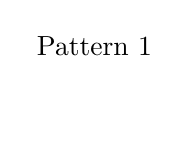
\begin{tikzpicture}
            \node [] (n0)  at (0.0,0.0) {};
            \node [] (n1)  at (0.0,1.0) {Pattern 1}; 
        \end{tikzpicture} 
        &
        \begin{tikzpicture}
            \node [] (n1)  at (0.0,2.0) {$T_1 \rightarrow R_1$}; 
            \node [] (n2)  at (1.8,1.0) {$T_2 (= R_1) \rightarrow R_2$};
            \node [] (n3)  at (4.2,0.0) {$T_3 (= R_2) \rightarrow R_3$}; 
            \draw[->] (0.5,1.7) -- (0.5,1.3);
            \draw[->] (3.0,0.7) -- (3.0,0.3);
        \end{tikzpicture}

        \\
        \midrule
        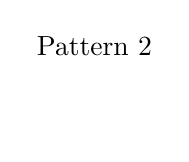
\begin{tikzpicture}
            \node [] (n0)  at (0.0,0.0) {};
            \node [] (n1)  at (0.0,1.0) {Pattern 2}; 
        \end{tikzpicture} 
         &
        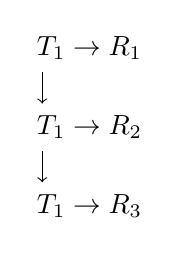
\begin{tikzpicture}
            \node [] (n1)  at (0.0,2.0) {$T_1 \rightarrow R_1$}; 
            \node [] (n2)  at (0.0,1.0) {$T_1 \rightarrow R_2$};
            \node [] (n3)  at (0.0,0.0) {$T_1 \rightarrow R_3$}; 
            \draw[->] (-0.6,1.7) -- (-0.6,1.3);
            \draw[->] (-0.6,0.7) -- (-0.6,0.3);
        \end{tikzpicture}

        \\
        \midrule
        \begin{tikzpicture}
            \node [] (n0)  at (0.0,0.0) {};
            \node [] (n1)  at (0.0,2.0) {Pattern 3}; 
        \end{tikzpicture} 
        &
        \begin{tikzpicture}
            \node [] (n0)  at (2.2,4.0) {$[T]$}; 
            \node [] (n1)  at (0.0,3.0) {$T_1 \rightarrow R_1$}; 
            \node [] (n2)  at (1.8,2.0) {$T_2 \rightarrow R_2$};
            \node [] (n3)  at (4.2,1.0) {$T_3  \rightarrow R_3$}; 

            \draw[->] (n0.south) -- (-0.5,3.3);
            \draw[->] (n0.south) -- (1.3,2.3);
            \draw[->] (n0.south) -- (3.5,1.3);
        \end{tikzpicture}

        \\
        \midrule

        \begin{tikzpicture}
            \node [] (n0)  at (0.0,0.0) {};
            \node [] (n1)  at (0.0,2.0) {Pattern 4}; 
        \end{tikzpicture} 
        &
        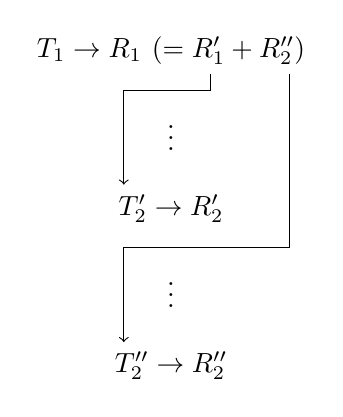
\begin{tikzpicture}
            \node [] (n0)  at (0.0,4.0) {$T_1 \rightarrow R_1\textit{ }( = R_1^\prime + R_2^{\prime\prime} )$}; 
            \node [] (d0)  at (0.0,3) {$\vdots$}; 
            \node [] (n1)  at (0.0,2) {$T_2^\prime \rightarrow R_2^\prime$}; 
            \node [] (d0)  at (0.0,1) {$\vdots$}; 
            \node [] (n2)  at (0.0,0.0) {$T_2^{\prime\prime} \rightarrow R_2^{\prime\prime}$};
            \draw [->] (0.5, 3.7) -- (0.5, 3.5) -- (-0.6, 3.5) -- (-0.6, 2.3);
            \draw [->] (1.5, 3.7) -- (1.5, 1.5) -- (-0.6, 1.5) -- (-0.6, 0.3);
        \end{tikzpicture}
        \\
        \bottomrule
        \end{tabular}
    \end{center}
    \caption{Coherence patterns that are defined by \newcite{danes74a}. A horizontal arrow indicates a transition in an utterance, while a vertical one indicates a contextual connection within utterances.}
    \label{tab:danesh_coherence_patterns}
\end{table}
%
\newcite{danes74a} interprets these patterns as follows:

\begin{itemize}
\item Pattern 1: This patterns illustrates a linear transition between themes and rhemes. 
In this pattern, each text unit takes the rheme presented in the preceding context of the unit as given information and transfers it to new information or a new rheme. 
In other words, each R (i.e.\ new information) in a text unit becomes T (i.e.\ given information) in its next unit.  


\item Pattern 2: 
This pattern depicts a constant theme continuation across text units.  
One theme appears in a series of text units, each of which, however, presents new information about the presented theme. 


\item Pattern 3: 
In this pattern, $[T]$ indicates a hypertheme, which is a global theme of a text unit.  
This pattern shows that different units can be connected because their themes, or their given information, are semantically related to a hypertheme. 

\item Pattern 4: 
Different combinations of patterns can emerge in different texts. 
Some of such combinations are such frequent that they can be taken as particular types of \mbox{theme-rheme} transitions of a higher order. 
This pattern is one of the most high-order patterns, where a text unit presents two (which can in potential be several) rhemes, $R^\prime$ and $R^{\prime\prime}$, in connection with a given theme. 
First, $R^{\prime}$ is expounded, and when its progression completes, $R^{\prime\prime}$ becomes the theme for another transition. 
 In-between transitions for extending each rheme may follow their own patterns. 
\end{itemize}

\newcite{danes74a} brings this point to the attention that one of the crucial properties of these patterns is their missing link.   
For example, in Pattern 1 there is no link between the earliest and latest text units. 
Those are connected because of the middle unit that makes transitions between themes and rhemes smoother. 
In contrast, all text units in Pattern 3  are linked to each other because they all have $T_1$ as shared given information. 

\section{Evaluation}
\label{sec:coh-eval}

The goal of the research presented in this dissertation is to provide an approach to coherence modeling and compare it with other models. 
In order to accomplish this, it is essential to have a method to evaluate the performance of coherence models. 
In this section, we complete our definition by describing the evaluation methods we employ for assessing coherence models that are examined in our experiments. 

\subsection{Intrinsic vs. Extrinsic}

Intrinsic and extrinsic are two types of evaluation methodologies for computational methods.  
In an intrinsic evaluation, system outputs are directly evaluated in terms of a set of norms or predefined criteria about the desired functionality of the system itself. 
In an extrinsic evaluation, system outputs are assessed on their impacts on a task external to the system itself. 

Some research papers on local coherence modeling use intrinsic evaluation approaches such as sentence ordering \cite{lapata03, mihalcea04b, karamanis04a, barzilay04, barzilay08}. 
Such an evaluation method is primarily designed to model violations of restrictions in the centering theory \cite{karamanis04a}. 
The goal of the sentence ordering task is to check if a coherence model can recognize the original order of sentences in a text as the best order of its sentences. 
The main underlying assumption for this task is that perturbing the order of sentences in a text disturbs its coherence.  
However, this task is too artificial and not suitable for evaluating the coherence of text \cite{lai18}.  

Some other approaches take the coherence of a text as a factor of the text quality and extrinsically evaluate the coherence model in downstream tasks \cite{miltsakaki04a,yannakoudakis12}. 
In this dissertation, we follow extrinsic evaluation methods, and evaluate our coherence model based on its performance for the readability assessment task and the automatic single document summarization task.  

In the readability assessment task  \cite{miltsakaki00,pitler08,petersen09,flor13}, a coherence model is used to assess the readability of texts. 
The insight of this task is that coherent texts are less complicated than other ones; therefore, they are easy to read and understand \cite{pitler08}. 
We take readability assessment as an extrinsic evaluation task for coherence models because there are many other text characteristics that influence readability.  

Automatic summarization has been receiving enormous attention by researchers in natural language processing because of its potential for various information access applications. 
For instance, it is useful for tools that aid users to navigate and digest web content (e.g.\ news, social media, product reviews), question answering, and personalized recommendation engines. 
Single document summarization is the task of producing a shorter version of a text while preserving its information content \cite{nenkova11}. 
A basic approach to single document summarization is extractive, in which a summary is produced by identifying and concatenating the most important sentences in a text. 
Ideally, information in selected sentences for a summary should be the most important information in the input text. 
This information, however, should have satisfactory variance (or minimum redundancy), and be presented coherently in the summary to be readable. 
Developing an extractive summarizer that jointly optimizes these three crucial factors -- importance, diversity, and coherence -- is a challenging task because the inclusion of relevant sentences relies not only on properties of the sentences themselves, but also the properties of every other sentence in a summary. 
Moreover, since the length of a summary is limited\footnote{Forcing summaries to obey a length constraint is a typical setup in summarization as it allows for a fair empirical comparison between different possible outputs. 
 Furthermore, it represents a real world scenario where summaries are supposed to be shown on small screens. 
}, making a balance between these three factors is difficult. 
For example, a summarizer may select a sentence which contains less important information in comparison to other sentences just to make other selected sentences coherent. 

\subsection{Ranking as Classification} 

Coherence is not a binary property of a text that either exists or not. 
It is a comparative attribute of texts: Is a text more coherent than other one? 
Even for humans, it might be ambiguous to decide if a text is coherent or not; however, they can rank texts with respect to their coherence \cite{halliday76}. 
This fits to the task of text ranking with respect to readability, where a coherence model is evaluated by comparing its rankings with rankings provided by humans for readability. 

From the computational point of view, the core of the evaluation method in this dissertation is a pairwise ranking task: Given a pair of texts, which one is more coherent? 
For being convenient for machine learning models, the pairwise ranking task is recast as a classification task, where each text pair is associated with a label. 
The value of the label represents which text in a pair should be ranked higher; we use label $+1$ where the first text in a pair is ranked higher, and $-1$ otherwise. 
This binary classification task can be solved by a machine learning approach, such as Support Vector Machines (SVMs) \cite{bishop06}.  
The details of experimental setups for machine learning models are explained in Chapter~\ref{ch:coh-patterns} and Chapter~\ref{ch:lex-graph}.  

\subsection{Evaluation Metrics}

In order to perform a quantitative analysis of labels predicted by a coherence model for text pairs, we employ different metrics.

For the readability assessment task we use accuracy and F1-measure. 
Accuracy quantifies how often a coherence model makes a correct decision on text pairs in test data.
A decision is correct if the label predicted by a model for a text pair is identical with the label that is assigned by human judges.

F1-measure is the harmonic mean between precision and recall. 
Precision is the ratio of the number of correct predictions over the number of all predicted labels. 
If a model predicts a label for each text pair in test data, then precision and accuracy are identical. 
However, it is also likely that a model does not rank a pair of texts and sees the texts equally coherent.  
In such cases, precision and accuracy are not identical.    
Recall is the number of correct predictions among the number of pairs with the desired label in test data. 

For the summarization task, we use ROUGE metrics to evaluate the performance of the examined summarizers. 
ROUGE is a standard metric for text summarization. It compares a summary generated by a summarizer with a gold summary, which usually is generated by a human, based on word overlaps between summaries. 
We explain these metrics in more details in related chapters of this thesis. 

